%%
%% Template thesis.tex
%%

% \documentclass[twoside,doublespace,onecolumn,11pt,a4paper]{book}
% \usepackage[palatino]{StyFiles/anuthesis}
% \usepackage{StyFiles/thesis}
% \usepackage{makeidx}
% \usepackage[toc,page]{appendix}
% \usepackage{StyFiles/fancyhdr}

\documentclass[conference,compsoc]{IEEEtran}
\usepackage{graphicx}
% \usepackage{StyFiles/doublespace}

% Chuck Added
% Gould Configurations

% For figures
% \ifCLASSINFOpdf
% \usepackage[pdftex]{graphicx}
% \DeclareGraphicsExtensions{.jpg,.png}
% \else
% \usepackage[dvips]{graphicx}
% \DeclareGraphicsExtensions{.eps}
% \fi

% For citations
\usepackage[sort,numbers]{StyFiles/natbib}
\renewcommand{\citename}{\citet}
\renewcommand{\cite}{\citep}
\usepackage{StyFiles/natbibspacing}

% For maths
\usepackage[cmex10]{amsmath}
\usepackage{amssymb,amsthm}

% For algorithms
\usepackage{StyFiles/algorithm}
\usepackage{StyFiles/algorithmic}

% For Hyperlinks
\usepackage{hyperref}
% fix problem between hyperref and algorithmic
\newcommand{\theHalgorithm}{\arabic{algorithm}}

% For captions
\usepackage[font=small,labelfont=bf]{caption}
\usepackage[font=footnotesize]{subfig}

% My macros
\usepackage{StyFiles/sg-macros}

\newtheorem{thm}{Theorem}[section]
\newtheorem{cor}[thm]{Corollary}
\newtheorem{lem}[thm]{Lemma}
\newtheorem{prop}[thm]{Proposition}
\newtheorem{obs}[thm]{Observation}
\newtheorem{defn}[thm]{Definition}

\newcommand{\mmqp}[3]{\textrm{\sc MaxMarginQP}\!\left(\{\by_t, #1\}_{t=1}^{T}, #2, #3\right)}

\makeatletter
\setlength\@fptop{0pt} 
\setlength\@fpsep{8pt plus 1fil} 
\setlength\@fpbot{0pt}
\makeatother
% % correct bad hyphenation here
% \usepackage{StyFiles/hyphenat}
% \hyphenation{op-tical net-works semi-conduc-tor}


%%%%%%%%%%%%%%%%%%%%%%%%%%%%%%%%%%%%%%%%%%%%%%%%%%%%%%%%%%%%%%%%%%%%%%%
%% Preamble
% \title{Latent Structural SVM Learning for Lower Linear
%   Envelope Potentials in Binary Markov Random Fields}
% \author{Chang Li} \date{\today}

% \renewcommand{\thepage}{\roman{page}}

% \makeindex

\begin{document}
\title{A New Method for Stock Price Prediction Based on MRFs and SSVM}


% author names and affiliations
% use a multiple column layout for up to three different
% affiliations
\author{\IEEEauthorblockN{Anonymous}}

% conference papers do not typically use \thanks and this command
% is locked out in conference mode. If really needed, such as for
% the acknowledgment of grants, issue a \IEEEoverridecommandlockouts
% after \documentclass

% for over three affiliations, or if they all won't fit within the width
% of the page (and note that there is less available width in this regard for
% compsoc conferences compared to traditional conferences), use this
% alternative format:
% 
%\author{\IEEEauthorblockN{Michael Shell\IEEEauthorrefmark{1},
%Homer Simpson\IEEEauthorrefmark{2},
%James Kirk\IEEEauthorrefmark{3}, 
%Montgomery Scott\IEEEauthorrefmark{3} and
%Eldon Tyrell\IEEEauthorrefmark{4}}
%\IEEEauthorblockA{\IEEEauthorrefmark{1}School of Electrical and Computer Engineering\\
%Georgia Institute of Technology,
%Atlanta, Georgia 30332--0250\\ Email: see http://www.michaelshell.org/contact.html}
%\IEEEauthorblockA{\IEEEauthorrefmark{2}Twentieth Century Fox, Springfield, USA\\
%Email: homer@thesimpsons.com}
%\IEEEauthorblockA{\IEEEauthorrefmark{3}Starfleet Academy, San Francisco, California 96678-2391\\
%Telephone: (800) 555--1212, Fax: (888) 555--1212}
%\IEEEauthorblockA{\IEEEauthorrefmark{4}Tyrell Inc., 123 Replicant Street, Los Angeles, California 90210--4321}}




% use for special paper notices
%\IEEEspecialpapernotice{(Invited Paper)}




% make the title area
\maketitle

% As a general rule, do not put math, special symbols or citations
% in the abstract
\begin{abstract}

  Trading strategies basing on both financial analysis and
  machine learning techniques are becoming increasingly popular
  due to their ability to capture micro market price movements
  and leverage big data. An important class of works are focusing
  on exploiting the structural relationships between companies
  for accurate stock price prediction. In this paper we develop
  an algorithm for learning the parameters of unary and binary
  potentials in binary markov random fields (MRFs) under the
  max-margin framework. We first show how to train unary
  potentials using market price data and Gaussian Mixture Models
  (GMMs). Then, we developed a graph-cut based algorithm to solve
  the inference problem exactly. We demonstrate the learning of
  potentials' parameters using a max-margin learning framework.
  Experiment is conducted by comparing performances between our
  formulation and conventional SVM method. Results show that our
  method outperforms SVM by 27.9\% on train set and 40.5\% on
  test set.

 \end{abstract}

% no keywords




% For peer review papers, you can put extra information on the cover
% page as needed:
% \ifCLASSOPTIONpeerreview
% \begin{center} \bfseries EDICS Category: 3-BBND \end{center}
% \fi
%
% For peerreview papers, this IEEEtran command inserts a page break and
% creates the second title. It will be ignored for other modes.
\IEEEpeerreviewmaketitle



% \pagenumbering{roman}  % first use Roman numerals for page numbers

% %%%%%%%%%%%%%%%%%%%%%%%%%%%%%%%%%%%%%%%%%%%%%%%%%%%%%%%%%%%%%%%%%%%%%%%
% %% Title page
% \pagestyle{empty}
% \thispagestyle{empty}
% %% Template titlepage.tex
%%
%% anuthesis.sty Copyright (C) 1996, 1997 Steve Blackburn
%%
%% Department of Computer Science, Australian National University
%%

\begin{titlepage}
  \enlargethispage{2cm}
  \begin{center}
    \makeatletter
    \Huge\textbf{\@title} \\[.4cm]
    \Huge\textbf{\thesisqualifier} \\[2.5cm]
    \huge\textbf{\@author} \\[8.5cm]
    \makeatother
    \Large A subthesis submitted in partial fulfillment of the degree of \\
    \LARGE Master of Science (Honours) at \\
    The Department of Computer Science\\
    Australian National University \\[2cm]
    \thismonth
  \end{center}
\end{titlepage}

%%% Local Variables: 
%%% mode: latex
%%% TeX-master: "thesis"
%%% End: 


% %%%%%%%%%%%%%%%%%%%%%%%%%%%%%%%%%%%%%%%%%%%%%%%%%%%%%%%%%%%%%%%%%%%%%%%
% %% Here begin the preliminaries
% %%
%% Template frontmatter.tex (Copyright etc.)
%%

\vspace*{14cm}
\begin{center}
  \makeatletter
  \copyright\ \@author
  \makeatother
\end{center}
\noindent
\begin{center}
  \aboutthesis
\end{center}
\noindent

\newpage

\vspace*{7cm}
\begin{center}
  Except where otherwise indicated, this thesis is my own original
  work.
\end{center}

\vspace*{4cm}

\hspace{8cm}\makeatletter\@author\makeatother\par
\hspace{8cm}\today


%%% Local Variables: 
%%% mode: latex
%%% TeX-master: "thesis"
%%% End: 


% %%%%%%%%%%%%%%%%%%%%%%%%%%%%%%%%%%%%%%%%%%%%%%%%%%%%%%%%%%%%%%%%%%%%%%%
% %% Dedication (optional)
% \cleardoublepage
% \pagestyle{empty}
% %%
%% Template dedication.tex
%%

\vspace*{7cm}
\begin{center}
  To my parents.
\end{center}


%%% Local Variables: 
%%% mode: latex
%%% TeX-master: "thesis"
%%% End: 



% %%%%%%%%%%%%%%%%%%%%%%%%%%%%%%%%%%%%%%%%%%%%%%%%%%%%%%%%%%%%%%%%%%%%%%%
% %% Acknowledgements (optional!)
% \cleardoublepage
% \pagestyle{empty}
% %%
%% Template ack.tex
%%

\chapter*{Acknowledgements}
\label{cha:ack}
\addcontentsline{toc}{chapter}{Acknowledgements}

I would like to express my very great appreciation to my
supervisor Stehpen Gould for his valuable and constructive
suggestions during the planning and development of this
research work. His great patience and willingness to give
his time so generously has been very much appreciated.

I would also like to express my very great appreciation to the
open source community (Python, OpenCV and Chun-Nam Yu etc.). I
cannot finish this work without their generous contributions.

%%% Local Variables: 
%%% mode: latex
%%% TeX-master: "thesis"
%%% End: 



% %%%%%%%%%%%%%%%%%%%%%%%%%%%%%%%%%%%%%%%%%%%%%%%%%%%%%%%%%%%%%%%%%%%%%%%
% %% Abstract
% \cleardoublepage
% \pagestyle{headings}
% %%
%% Template abstract.tex
%%

\chapter*{Abstract}
\label{cha:abstract}
\addcontentsline{toc}{chapter}{Abstract}

The lower linear envelope potentials, one of higher-order
potentials used in Markov Random Fields (MRFs) are raising
interests in recent years due to its capability of enforcing
consistency over large sets of random variables. Previous
researches in this area are only able to learn the lower linear
envelope function approximately thus losses a rich class of
representations which may harm the model's performance.

In this thesis we propose an exact formulation of the lower
linear envelope function which can also be inferred exactly and
learned using the latent structural SVM. We first show the
implicit equivalence between the quadratic pseudo-Boolean
formulation and linear combination formulation of the lower
linear envelope. Then, with the exact inference developed by
previous research~\cite{gouldlearning}, we propose the learning
algorithm based on the linear combination formulation within a
latent structural SVM framework.

We experiment our algorithm on two experiments and demonstrate
advantages and disadvantages between our new formulation and
previous formulation~\cite{gouldlearning,Gould:ICML2011}. The
results show that despite computational expensive during
training, our new method is more efficient during testing, able
to learn the lower linear envelope exactly and performs better on
harder problems than the previous method.


%%% Local Variables: 
%%% mode: latex
%%% TeX-master: "thesis"
%%% End: 


% %%%%%%%%%%%%%%%%%%%%%%%%%%%%%%%%%%%%%%%%%%%%%%%%%%%%%%%%%%%%%%%%%%%%%%%
% %% Table of contents
% \cleardoublepage
% \pagestyle{headings}
% \markboth{Contents}{Contents}
% \tableofcontents
% \listoffigures
% \listoftables

% \pagenumbering{arabic} % switch to Arabic numerals for page numbers
% \setcounter{page}{1}  % set page number to 1


%%%%%%%%%%%%%%%%%%%%%%%%%%%%%%%%%%%%%%%%%%%%%%%%%%%%%%%%%%%%%%%%%%%%%%%
%% Other options
% \begin{doublepage}

%%%%%%%%%%%%%%%%%%%%%%%%%%%%%%%%%%%%%%%%%%%%%%%%%%%%%%%%%%%%%%%%%%%%%%
%% Here begins the main text
% \mainmatter

%% Introduction
% %%
%% Template intro.tex
%%

\chapter{Introduction}
\label{cha:intro}

One interesting task in machine learning is labeling over complex
and structured objects. Many applications such as image
segmentation, motif finding and noun-phrase parsing involved with
representing jointly correlated variables. Encoding consistency
constraints over large number of random variables, for example,
is central to the problem of image segmentation. Algorithm
frameworks like Markov Random Field (MRF) containing higher order
energy functions and max margin method for solving learning
problem are raising interests recently due to their capability of
representing structural dependencies of variables and ensuring
computationally feasible approximation.
  
Lower linear envelope potentials is one of higher order energy
functions defined on MRF which becomes popular due to their
ability to encode consistency relationship between labels in
clique. \citename{gouldlearning} investigated the submodularity
of lower linear envelope potentials and developed a graph-cuts
algorithm to perform exact inference on them. Then they proposed
a Max-Margin framework to optimize potentials' parameters.
However, in order to write the energy function into a linear
combination, they sampled the lower linear envelope potentials
using a set of fixed space points. Althought this formulation can
be globally optimized by using the Max-Margin framework, it lost
a rich class of representations of energy function due to the
fixed space sampling. Removing the equally spaced constraint and
introduce their auxiliary variables back will result in a latent
SVM formulation. Under this formulation the algorithm can learn
the lower linear envelope exactly. Our main goal in this thesis
is focused on this extension. The difficulty is how to learn
parameters of energy function together with latent information.
  
In practical, many information providing useful cues for
prediction is not directly observable from data. For motif
(repeated patterns in DNA sequences) finding problem, as an
example, the task if to find motifs from a set of DNA sequences
where the location of these motifs are unknown. Thus the
information of position can be treated as hidden variable and is
important to be considered in the model though it is not directly
observable. Issues like this have been well studied by many
researchers and latent SVMs, which can explicitly model hidden
variables with joint feature vectors, outperforms many other
methods.
  
The latent SVM was developed by
\citename{felzenszwalb2008discriminatively} and
\citename{yu2009learning} independently in different ways. The
main idea is introducing a latent variable to extend the feature
vector, which results in an arbitrary loss function, e.g. Hinge
Loss, with an upper bound. Then the optimization was done by
using Concave-Convex Procedure (CCCP) algorithm, which is
guaranteed to decrease the objective function to a local minimum.
 
In this thesis, we are aiming at exploring a variant formulation
of \citename{gouldlearning} by rewriting the lower linear
envelope function directly into a linear combination and
developing the learning algorithm using the latent structural
SVM. The rest of the thesis is structured as follows:

Chapter~\ref{cha:RelatedWorks} describes work related to MRFs and
latent structural SVM. We also provide some background about our
experiments. 

Chapter~\ref{cha:methodology} describes our main contributions.
We first introduce the concept of the lower linear envelope and
the exact inference method developed by \citename{gouldlearning}.
We then propose the exact formulation of the lower linear
envelope and develop the learning algorithm basing on that
formulation. 

Chapter~\ref{cha:Experiments} describes two experiments we use to
compare our new method to previous method~\cite{gouldlearning}.
We also give brief explanations and summary at the end of each
experiments. 

Chapter~\ref{cha:conclusion} summarizes our work and point out
advantages and disadvantages of our new formulation. We also
provide some insights for future work.

%%% Local Variables: 
%%% mode: latex
%%% TeX-master: "thesis"
%%% End: 


%% Chapters
% \section{Background for Experiments}

% \subsection{Superpixel}
% \label{sec:superpixel}

% \begin{figure}[t]
%   \centering
%   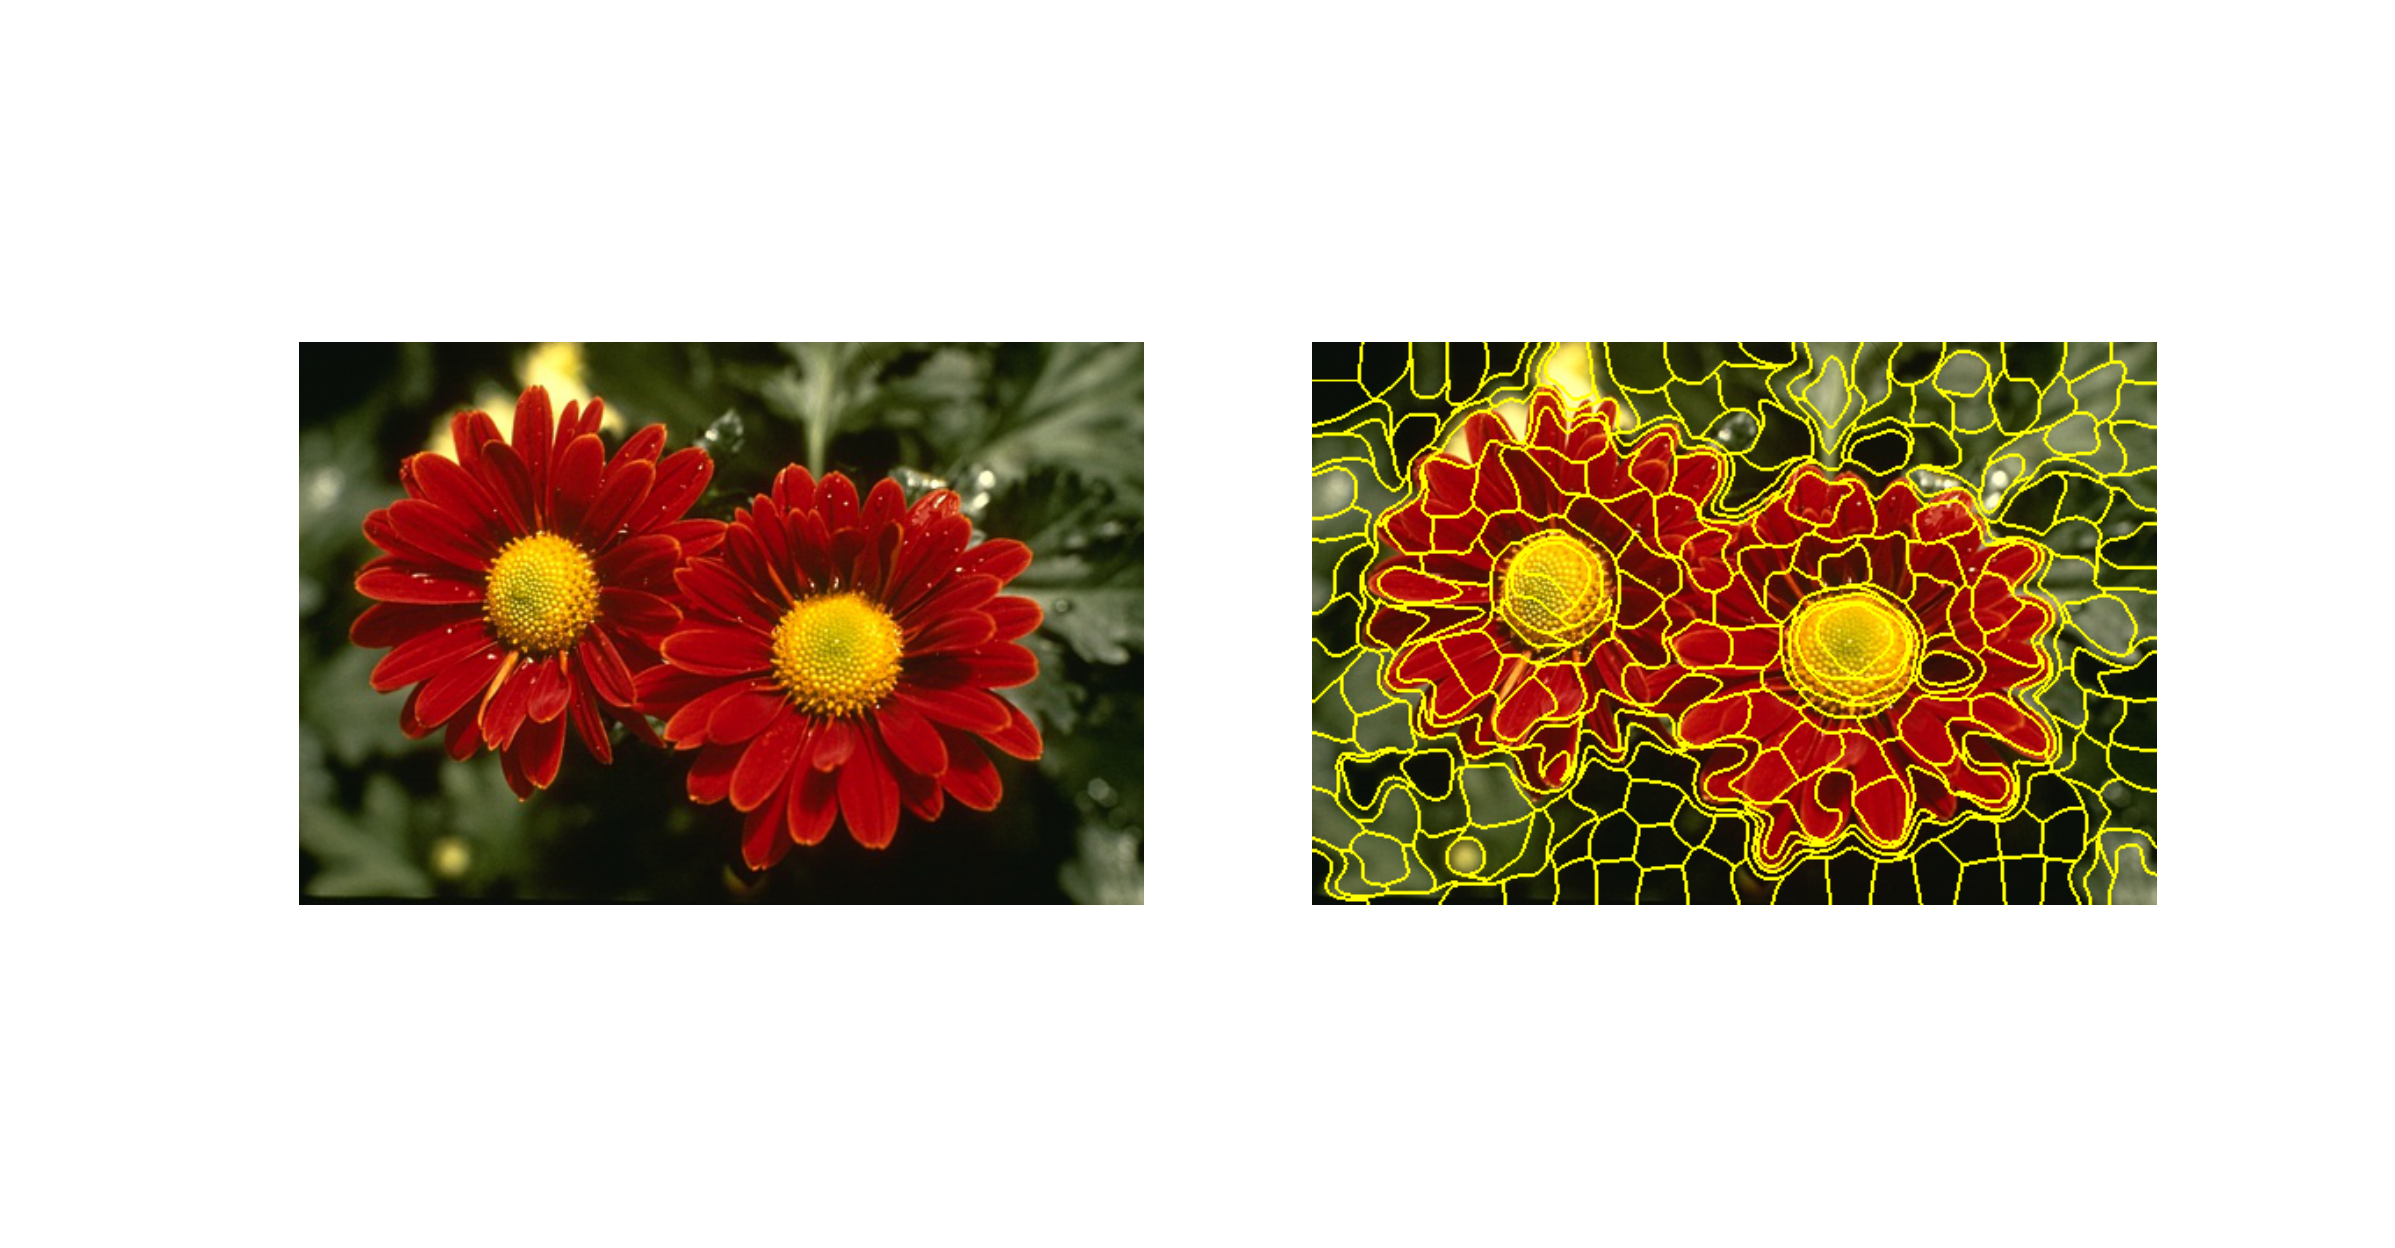
\includegraphics[width=1\linewidth]{RelatedWorks/figures/Flower_Origin_Segment.png}
%   \caption{\label{fig:superpixel_example} Picture on the left is
%     the original picture which contains 154,400 pixels. Picture
%     on the right is the same picture represented by 268 superpixels}
% \end{figure}

% Markov Random Fields are often defined on grids of pixels or
% ``cliques''. However, artificial pixel-grids are usually
% computational expensive and not natrual representations of
% images. A much preferable representation is to group images in a
% both perceptual and semantic meaningful way. Superpixel
% algorithms, by capturing redundancy in images, can group pixels
% into semantically meaningful homogeneous regions and reduce
% hundreds of thousands of pixels into several hundreds of
% superpixels (see figure~\ref{fig:superpixel_example}). Such a superpixel map can greatly increase the
% efficiency of images processing tasks by providing an efficient
% primitive on which MRF can compute
% Energies\cite{achanta2012slic}.

% There are various superpixel segmentation algorithms. When
% choosing the desirable algorithm we mainly consider the following
% two aspects\cite{achanta2012slic}:

% \begin{enumerate}
% \item Computational Efficiency: Superpixels should be fast to
%   generate. Algorithms with less complexity are much preferable.
% \item Adherence to boundaries: Algorithms which can generate
%   superpixels with higher boundary recall (less true edges are
%   missed) are much preferable.
% \end{enumerate}

% Basing on those two considerations the superpixel algorithm we use
% in this thesis is the state-of-the-art \emph{Simple Linear
%   Iterative Clustering} (SLIC) algorithm which out-performs other
% algorithms in nearly all aspects\cite{achanta2012slic}. SLIC in
% essence is an adaptation of $k$-means clustering algorithm. It
% mainly differs from $k$-means with two
% distinctions\cite{achanta2012slic}:

% \begin{figure*}[h]
%     \centering
%     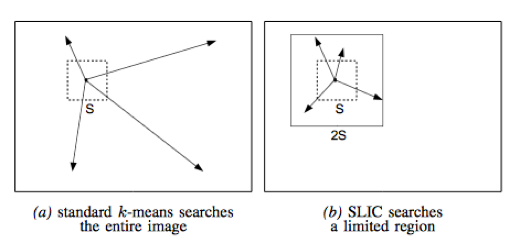
\includegraphics[width=0.8\linewidth]{RelatedWorks/figures/SLIC_AssignStep.png}
%     \caption{\label{fig:SLIC_Regions}SLIC narrows the superpixel
%       search regions.}
% \end{figure*}

% \begin{enumerate}
% \item Searching space: In the assignment step $k$-means
%   clustering computes distances from each cluster to every pixel
%   in the image. On the other hand SLIC narrow the search space
%   into a $2S\times 2S$ region (see figure~\ref{fig:SLIC_Regions}), where $S=\sqrt{\frac{N}{K}}$. $N$
%   is the number of total pixels in images and $k$ is the only
%   parameter of the algorithm which defines the number of
%   superpixels (clusterings). Therefore, the SLIC algorithm
%   reduces the complexity from $k$-means' $\mathcal{O}(N^k)$ to a
%   linear complexity $\mathcal{O}(N)$.

% \item Distance measurement: Distance in $k$-means algorithm is
%   measured by Euclidean norm of color vectors between pairs of
%   pixels. SLIC algorithm also takes spatial distance into account
%   by redefining the distance as $D =
%   \sqrt{d_c^2+(\frac{d_s}{S})^2m^2}$ where $d_c$ is the Euclidean
%   norm of color vectors and $d_s$ is the Euclidean norm of pixels'
%   positions. $m$ is a constant which indicates the relative
%   importance between color distance and spatial distance and thus
%   balances the compactness and adherence to boundries in
%   generated superpixels.
% \end{enumerate}

% In this thesis we use SLIC as our cliques generating algorithm
% because it is fast to compute and out-performs other algorithms
% on adherence to image boundries while keeping results compact.

\subsection{GrabCut}
\label{sec:grabcut}

\begin{figure}[b]
  \centering
  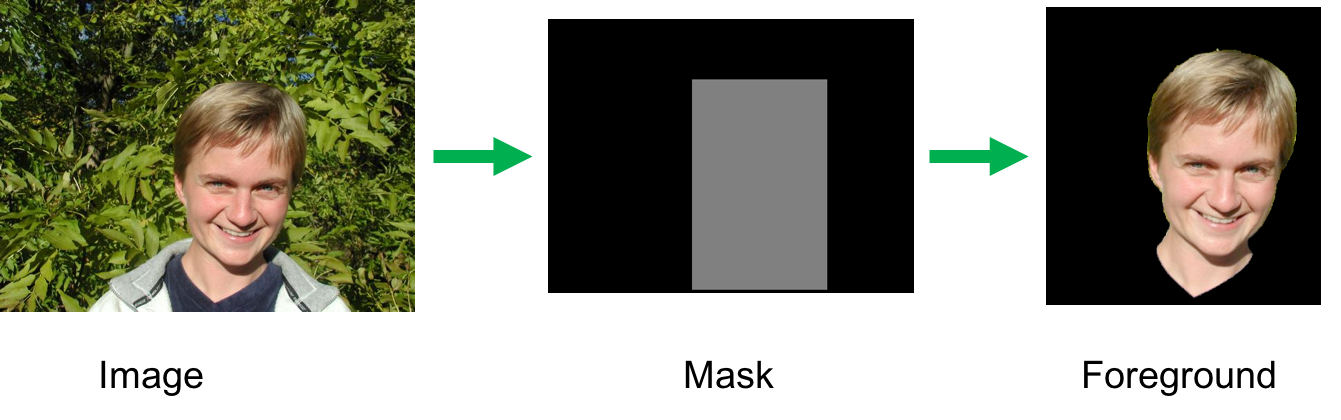
\includegraphics[width=1\linewidth]{RelatedWorks/figures/grabcut_task.png}
  \caption{\label{fig:grabcut_example} Picture on the left is
    the original picture. Picture
    on the middle is a user defined mask. The task is to extract
    foreground pixels within that rectangle. On the right is the
    ground truth foreground.}
\end{figure}

\emph{GrabCut} algorithm was proposed
by~\citename{Rother:SIGGRAPH04} in order to solve background
foreground segmentation problem (see
figure~\ref{fig:grabcut_example}). They first defined MRFs over
an labeled image and then use
\emph{graph-cuts}~\cite{Boykov:ICCV01} method to do the
inference. In this section we mainly focus on two of their
contributions: estimating color distribution (foreground and
background) using \emph{Gaussian Mixture Models} (GMMs) and an
\emph{EM} like two-step algorithm to train their model.

Suppose there are $N$ pixels in an image. In order to construct
MRFs, they first defined an energy
function~\eqref{eq:energyfunction_UPH} with unary and pairwise
terms:

\begin{align}
  \label{eq:grabcut_energy}
  E(\alpha, \bk, \btheta, \bz) = 
  \sum_{i\in \N}{\phi^U(\alpha_i, \bk_i, \btheta, \bz_i)}+
  \sum_{(i,j)\in \E}{\phi^P(\alpha_i,\bz_i)}
\end{align}
where $i$ is the index of pixels, $\alpha \in {0,1}$ is the label
for pixel $i$. $0$ is for the background and $1$ is for the
foreground. $\bz$ denotes the pixel vector in RGB color space.
$\bk$ and $\btheta$ are all parameters vectors and will be
explained in the next paragraph. 

The first contribution is using \emph{Gaussian Mixture Models}
(GMMs) with $K$ components (typically $K=5$) for generating unary
terms. They used two GMMs in their model, one for background and
one for foreground. $\bk={\bk_1,\dots,\bk_i,\dots,\bk_N}$ with
$\bk_i\in 1,\dots,K$ assigns each pixel $i$ to a unique GMMs
component. The component is either belonging to background's GMMs
or foreground's GMMs, which is depended on the label $\alpha_i\in
{0,1}$. $\btheta$ is the parameter vector which contains
parameters of standard GMMs plus \emph{mixture weighting
  coefficients}~\cite{Rother:SIGGRAPH04}.

The pairwise function $\phi^P$ is defined as a smoothness
indicator which measures both color space and spatial distances
simultaneously. It is used to encourage coherence of similar
pixel pairs. This energy function was later used to construct an
\emph{st min-cut} graph which can be inferred efficiently using
\emph{graph-cuts}~\cite{Boykov:ICCV01} algorithm. This gives some
insights to their second contribution.

To optimize the performance, they developed a two-step learning
algorithm. The algorithm first re-assign GMMs components ($\bk$)
to each pixel then update parameters $\btheta$ with new
assignments. The result of the trained GMMs are used directly
into \emph{graph-cuts} algorithm as unary terms. Finally the
label $\alpha_i$ for each pixel $i$ is inferred jointly using
\emph{graph-cuts} algorithm. This whole procedure is repeated
until convergence (or reaches termination conditions). We briefly
summarized this procedure in \algref{alg:grabcut}

\begin{algorithm}[tb]
  \begin{algorithmic}[1]
    \REPEAT
    \STATE{\emph{Assign GMM components} to pixels: \\
      $\bk_i^*=\argmin_{\bk_i}\phi^U(\alpha_i, \bk_i, \btheta,
      \bz_i)$}
    \STATE{\emph{Learn GMM parameters} from data z:\\
      $\btheta=\argmin_{\btheta}\sum_{i\in \N}{\phi^U(\alpha_i, \bk_i, \btheta, \bz_i)}$}
    \STATE{\emph{Estimate segmentation}: graph-cuts inference:\\
      $\min_{\alpha}\min_{\bk}E(\alpha, \bk, \btheta, \bz)$}
    \UNTIL{convergence}
  \end{algorithmic}
  \caption{\label{alg:grabcut} GrabCut training algorithm}
\end{algorithm}

In this thesis we also use GMMs trained by GrabCut algorithm for
our unary terms.


%%% Local Variables:
%%% mode: latex
%%% TeX-master: "../thesis"
%%% End:

\input RelatedWorks/RelatedWorks
\input Methodology/Methodology
\input Experiments/Experiments

% %% Conclusion
% %%
%% Template conclusion.tex
%%

\chapter{Conclusion and Future Work}
\label{cha:conclusion}

We summarize our work in this chapter. We will also conclude its
advantages and disadvantages basing on our synthetic
(section~\ref{sec:synth-check}) and real-world
(section~\ref{sec:foregr-extr}) experiments' results. Our work
also provide some insights to our future work which we will
briefly discuss in this chapter.


\section{Conclusion}
\label{sec:conclusion}

Lower linear envelope binary MRFs are raising interests due to
its capability for encoding higher-order consistency constraints
over large sets of random variables. \citename{gouldlearning} has
shown how to perform exact inference and learning of this problem
under the max margin framework. In order to transform the lower
linear envelope function to a linear combination formulation,
they interpolates it with a set of fixed space sample points.
Thus their algorithm is only able to learn the shape of the lower
linear envelope function approximately.

The main goal of our research is to learn the lower linear
envelope function exactly. Based on their work, we explore a
variant of their formulation by introducing auxiliary variables
back to the energy function to formulate an exact representation.
We find that the lower linear envelope function under the
quadratic pseudo-Boolean formulation~\eqref{eq:originalenergy}
itself is an inner product of parameters and features thus can be
written into a linear combination directly. Under this
formulation the inference algorithm (\emph{st min cut}
construction) developed by \citename{gouldlearning} still adapts
to our problem. Therefore, we are still able to conduct exact
inference on our problem. We developed the learning
\algref{alg:learning} using an extension of the max margin
framework which is known as latent structural SVM. However, this
algorithm is only guaranteed to decrease the objective function
to a local minimum thus the initial point will affect the overall
performance. In order to overcome this issue we also proposed an
empirical initialization \algref{alg:init_theta}.

In order to examine the effectiveness of our new algorithm, we
repeat two experiments \citename{gouldlearning} conducted in
their research and compare both results. In the first synthetic
checkerboard experiment, we found that in general the new
algorithm's accuracy is at least as well as the previous one. But
on harder problem~\ref{sec:unif-distr-squar} the new method
outperforms previous one significantly. The new method is much
more computationally expensive during the training period.
However it is more efficient during the testing stage because of
the simplicity of the shape of the lower linear envelope. We also
found that the shape learned by the new method can shift along
with the changes of the input data which proves that we can learn
the lower linear envelope exactly.

We then take our algorithm to a harder real-world
experiment~\ref{sec:foregr-extr}. It turns out that our new
method has a slightly increasing in overall accuracy (0.6\%)
compared to the previous method. There are much less holes in
images inferred by our new method which certificates the lower
linear envelope function learned by our formulation can better
enforce higher order consistency in large cliques. However, the
performance various significantly between cross-validation folds
which indicates there are some generalization issues existing in
our new method.

At last we summarize the advantages and disadvantages as
following.

\bigskip

Advantages of the new method (compared to the previous
method~\cite{gouldlearning,Gould:ICML2011}):

\begin{itemize}
\item Able to learn the lower linear envelope exactly.
\item Performs better (higher accuracy) on harder problems.
\item Efficient to compute during testing due to the simplicity
  of the shape of the lower linear envelope function.
\end{itemize}

Disadvantages of the new method:

\begin{itemize}
\item Only guaranteed to decrease to the local minimum.
\item Computationally expensive during training.
\item Generalization various significantly.
\end{itemize}




\section{Future Work}
\label{sec:futurework}

As we suggested in the conclusion, our new method seems to have
some generalization issues (figure~\ref{fig:grabcut_worst} for
example). It will be our primal goal to keep investigating into
this problem. We also proposed an empirical initialization method
in section~\ref{sec:mrflssvm_learning_algo}. For future work we
would compare this method to others.

Our research also provide insights to further directions.
Extending our approach to multi-label MRFs seems to be very
promising. Other straightforward extensions include the
introduction of features for modulating the higher-order terms
and the use of dynamic graph cuts~\cite{Kohli:PAMI07} for
accelerating loss-augmented inference within our learning
framework. Other optimization algorithms for solving our learning
problem may also be considered, \eg the subgradient
method~\cite{Nowozin:2011, Bertsekas:2004}.






%%% Local Variables: 
%%% mode: latex
%%% TeX-master: "thesis"
%%% End: 


%%%%%%%%%%%%%%%%%%%%%%%%%%%%%%%%%%%%%%%%%%%%%%%%%%%%%%%%%%%%%%%%%%%%%%
% Here begins the end matter

%%%
%% Template appendix.tex
%%

\appendix

\chapter{Some Other Stuff}
\label{app:app1}

\section{Why I Did It}
\label{sec:why3}

\chapter{More Stuff}
\label{app:app2}

%%% Local Variables: 
%%% mode: latex
%%% TeX-master: "thesis"
%%% End: 


% \backmatter

%%%%%%%%%%%%%%%%%%%%%%%%%%%%%%%%%%%%%%%%%%%%%%%%%%%%%%%%%%%%%%%%%%%%%%%
%% Other options
% \end{doublepage}

\bibliographystyle{abbrvnat}
\bibliography{Bibs/thesis,Bibs/long,Bibs/scene}

% \printindex

\end{document}

%%% Local Variables: 
%%% mode: latex
%%% TeX-master: "thesis"
%%% End: 



